\documentclass[titlepage]{article}

\usepackage[hidelinks]{hyperref}
\usepackage{stringstrings}
\usepackage[table]{xcolor}
\usepackage[english]{babel}
\usepackage{tabularx}
\usepackage[toc,page]{appendix}
\usepackage{gantt}
\setcounter{secnumdepth}{5}
\usepackage{tikz}
\usepackage{enumitem}
\usepackage{changepage}
\usepackage{colortbl}


\usetikzlibrary{automata, arrows, trees, positioning, fit, calc, shadows.blur, shapes.symbols}

\usepackage[top=1.5in, bottom=1.5in, left=2in, right=2in]{geometry}

\def\getfirstword#1{%
    \begingroup
    \edef\@tempa{#1\space}%
    \expandafter\endgroup
    \expandafter\readwords\@tempa\relax
}
\def\readwords#1 #2\relax{%
      \doword{#1}%  #1 = substr, #2 = rest of string
}
\def\doword#1{#1}
\def\endtestwords{}

\definecolor{navyblue}{RGB}{31,73,125}
\definecolor{burgundy}{rgb}{0.5, 0.0, 0.13}

\newcommand{\myparagraph}[1]{\paragraph{#1}\mbox{}\\}

\addtolength{\oddsidemargin}{-.875in}
\addtolength{\evensidemargin}{-.875in}
\addtolength{\textwidth}{1.75in}

\def \RoCM {Rotation Curve Modeler}
\def \SOCM {Scholarly Observed Celestial Measurements}
\def \RoCS {Rotation Curve Simulation}

\begin{document}

\title{
\textbf{
Software Requirements Specification}
\protect\\
for the
\protect\\
\textbf{
\RoCM\ (RoCM)}
\protect\\
{\small Version 2.0}}

\author{Robert Moss, Alex Clement
\protect\\
{\small Wentworth Institute of Technology}}
\maketitle

%%% Document Approval %%%
\section*{Document Approval}

The following Software Requirements Specification has been accepted and approved by the following:

\begin{center}
    \begin{tabularx}{\textwidth}{ |X|X|X|X| }
    \hline
    \textbf{Signature} & \textbf{Printed Name} & \textbf{Title} & \textbf{Date} \\ \hline
     &  &  &  \\ \hline
     &  &  &  \\ \hline
    \end{tabularx}
\end{center}

\newpage
\tableofcontents{} 
\newpage

\section{Introduction}

\subsection{Purpose}
The Software Requirement Specification for the Rotation Curve Modeler will explain in detail necessary features that the client purposes and the developers provide. Astrophysicists will be the main target for this web application. It will expedite the process of accessing galactic data (from the project Scholarly Observed Celestial Measurements) and provide a tool to model galaxies using many different theories to solve the rotation curve problem.

\subsection{Scope}
\begin{enumerate}
	\item Rotation Curve Modeler
	
  \begin{enumerate}	 	
    \item Interact with SOCM (Scholarly Observed Celestial Measurements)
	\begin{enumerate}
		\item Use the repository of observable galactic data to model hundreds/thousands of different galaxies.
	\end{enumerate}
    \item Interact with RoCS (Rotation Curve Simulation)
	\begin{enumerate}
		\item RoCS visualizes the spin of star clusters around the center of a galaxy. 
		\item Include scale and legend for the visualization.
	\end{enumerate}
    \item Allow users to locally import and run their own model (via JavaScript code)
	\begin{enumerate}
		\item Following the defined v(R) input/output standard.
		\item Observable galactic parameters from SOCM will be available as constants.
		\item User defined constants will need to be implemented in the user's function.
	\end{enumerate}
    \item Locally import LaTeX equation for each model (optional)
	\begin{enumerate}
		\item The user can import their own LaTeX equation to be displayed during the data plotting.
		\item Aids in understanding the behavior of each parameter.
	\end{enumerate}
	\item Dynamic parameter sliders
	\begin{enumerate}
		\item For every parameter in the individual models, a dynamic slider with user defined ranges can be created.
	\end{enumerate}
  \end{enumerate} 
  	\item rotationcurve.com / rotationcurve.org
    	\begin{enumerate}
        	\item The website will host the RoCM, SOCM, and ROCS components.
        	\begin{enumerate}
              \item This website, hosted on WIT servers, will allow astrophysicists to access a large database of observed galactic data (via SOCM), plot their own rotation curve models (via RoCM), and simulate their rotation curves (via RoCS).
        	\end{enumerate}
        \end{enumerate}
    
   
\end{enumerate}

\subsection{Definitions, Acronyms, and Abbreviations}
\begin{itemize}
	\item Application Specific Definitions
	\begin{itemize}
		\item RoCM - Rotation Curve Modeler
		\item SOCM - Scholarly Observed Celestial Measurements
		\item RoCS - Rotation Curve Simulator
	\end{itemize}
	\item Industry Definitions
	\begin{itemize}
		\item WIT - Wentworth Institute of Technology
		\item SRS - Software Requirements Specification
		\item JavaScript - A web based programming language.
		\item D3 - Data Driven Documents: A JavaScript library for data visualization.
		\item Ruby on Rails - A web development framework written in the Ruby programming language.
		\item JQuery - A JavaScript library for easy UI development.
		\item LaTeX - A document preparation system used widely throughout science and mathematics.
		\item SVG - Scalable Vector Graphics: A loss-less graphics format.
	\end{itemize}
	\item Technical Definitions
	\begin{itemize}
        \item MoND - Modification of Newtonian Dynamics
		\item TeVeS - Tensor-vector-scalar gravity
		\item MATLAB - A mathematical programming language (MATrix LABoratory).
		\item Mathematica - A mathematical programming language.
		\item DB - Database
        \item UI - User Interface
		\item GUI - Graphical User Interface
		\item HTML - HyperText Markup Language
		\item div - HTML tag to define a division in a document
        \item DOM - Document Object Model. A convention for representing and interacting with objects in HTML.
        \item API - Application Programming Interface
        \item km/s - Kilometers Per Second
        \item kpc - Kiloparsecs
	\end{itemize}
\end{itemize}

\subsection{References}
The list of references below are software documentation that we will be using:
\begin{enumerate}
	\item Data Driven Documents (D3): \href{http://d3js.org/}{\color{blue} http://d3js.org/}
	\item JQuery documentation: \href{http://api.jquery.com/}{\color{blue} http://api.jquery.com/}
	\item JQuery UI documentation: \href{http://api.jqueryui.com/}{\color{blue} http://api.jqueryui.com/}
\end{enumerate}

\subsection{Overview}
The rest of the SRS will contain:
\begin{enumerate}
	\item Specific features RoCM and the rotationcurve.org website
	\item System Requirements
	\item Design Constraints for the application.
	\item Risks within the scope.
	\item Any additional information about the development of the application.
\end{enumerate}

\section{General Description}
This section will explicitly lay out the product's functionality and constraints as well as compare it to existing products. Possible set backs will be discussed. Details about each requirement will be laid out in Section \ref{Specific Requirements}: \nameref{Specific Requirements}. 

\subsection{Product Perspective}
Astrophysicists will need to model galaxies in programs like MATLAB or Mathematica, but there doesn't exist a singular tool to expedite this process in a universal format. Currently, scholars must sift through peer-reviewed articles and gather data one-by-one. rotationcurve.org will help generalize the work being done on galaxy research and provide one central repository for researchers.

RoCM will serve as a visual modeler for our collections of data and contemporary theories within astrophysics. With observable data as the input (via SOCM), any galaxy can be imported into the tool. The tool will plot obervational data and multiple galactic models together as a graph, as well as enable users to import their own galatic models to test against existing theories. Sliders will allow users to control parameters within their models with realtime visual feedback in the generated graph.

\subsection{Product Functions}
There will be many available functions of RoCM users can utilize. The modular design of the software will allow for additional functions to be easily implemented.
\begin{enumerate}
	\item A rotation curve plotting tool that overlays different models of the galaxy on top of the observational data. Gives the user the ability to select which curve to plot based on the models available. Value ranged sliders that can update each individual parameter within specific galactic models. Each slider can be dynamically created with user defined ranges. This enables the user to visualize the behavior of each parameter within the each model. Allows for the testing of uncertainty within the galactic parameters.
	\item The rotationcurve.org website will provide a web interface to the RoCM, SOCM, and RoCS modules. The website back-end will host galaxy research data, namely through SOCM, which will also provide API endpoints for ease of access and extensibility. rotationcurve.org will provide an `About' section that explains the purpose of the website, and provides the email addresses to contact the contributors.
\end{enumerate}


\subsection{User Characteristics}
The rotationcurve.org website and its constituent modules will be targeted at researching astrophysicists in search of peer-reviewed galaxy data. Users will also benefit from the visualization features for their galactic rotation curve research. 

\subsection{General Constraints}
\label{General Constraints}
The D3 JavaScript library provides a fast an easy way to manipulate data and generate graphs in real time. Thus, it became our best option for rendering RoCM and RoCS. No detected flaws or deficiencies have been relevant to the project at this point, though we will be constrained by its capabilities for the duration of the project.

\subsection{Assumptions and Dependencies}
Users are expected to have the most updated versions of Google Chrome, or Mozilla Firefox. For the reasons stated in the \nameref{General Constraints} section, the chosen browser must have JavaScript enabled. An Internet connection is obligatory.

\section{Specific Requirements}
\label{Specific Requirements}
This section will explicitly lay out the purposed system design and it's individual requirements.

\subsection{External Interface Requirements}
\subsubsection{User Interfaces}
A web user interface will be developed to easily use the tools RoCM provides. A clean and clutter free UI will be necessary due to the complex nature of the physics involved (as to not overwhelm the user). If too much is incorporated as a part of the UI, the user will lose focus on the purpose of RoCM.

\subsubsection{Hardware Interfaces}
Users will need a device capable of supporting a modern browser and an Internet connection. Experience may depend on hardware capabilities and Internet speeds. No other external hardware dependencies are necessary.

\subsubsection{Software Interfaces}
RoCM will rely on the open source data visualization library D3.js (v3). A major software interfacing dependency will be JQuery 1.10.2, which will speed up the process of interfacing JavaScript with the HTML DOM elements. A LaTeX equation library, MathJax.js 2.3.1, will be used to convert raw LaTeX code into a formatted mathematical equation. An integration JavaScript library will be used for some of the galactic models. Other mathematical libraries will be added as needed.

\subsubsection{Communications Interfaces}
RoCM and RoCS will query data from the SOCM database. A bridge between the tools and the database will be developed to smoothly interface the front-end UI with the back-end data. A standardized format will be defined by SOCM.

\subsection{Functional Requirements}
\subsubsection{Rotational Curve Simulator (RoCM)}

\myparagraph{Introduction}
RoCM will serve as a visual modeler for our collection of data and contemporary theories for the solution to the rotation curve problem. With observable data as the input (via SOCM), any galaxy can be imported into the tool. The tool will plot obervational data and multiple galactic models together as a graph, as well as enable users to import their own galatic models to test against existing theories. Sliders will allow users to control parameters within their models with realtime visual feedback in the generated graph.

\myparagraph{Inputs}
RoCM will recieve it's galactic data from the SOCM API endpoints. For use of the sliders, users must click and drag JavaScript-generated sliders. The `LaTeX equation' section will require a properly-formed LaTeX equation (as dictated by the LaTeX standard) if the user desires to use the feature. The `JavaScript Model Input' section will require a properly-formed JavaScript function in the form v(R). Interaction with SOCM and RoCS will require mouse or cursor input.

\myparagraph{Processing}
Galactic data will be processed by the D3 JavaScript library, which generates and manipulates elements of the HMTL DOM to produce the graphs, sliders, and tables of RoCM. When the user changes the value of the sliders, each model that uses that parameter will be recalculated on the fly.

\myparagraph{Outputs}
RoCM produces a graph of Rotational Velocity (in km/s) over Galactocentric Distance (in kpc) with sliders to dynamically manipulate the graph.

\myparagraph{Error Handling}
If RoCM is unable to connect to SOCM, the page will detect the problem and issue an error message to the user. Errors resulting from JavaScript being disabled will be handled at a higher level (in the HMTL pages).

\subsubsection{rotationcurve.org Website}

\myparagraph{Introduction}
Currently, scholars must sift through peer-reviewed articles and gather galaxy data one-by-one. The rotationcurve.org website will help generalize the work being done on galaxy research and provide one central repository for researchers.

\myparagraph{Inputs}
Outside of the constituent modules of RoCMSOCM, the website will only require a user's mouse or cursor input for navigation. The website will be comprised of HTML, JavaScript, and CSS files. 

\myparagraph{Processing}
The web browser will process all necessary web requests and JavaScript will create the necessary navigational buttons on demand.

\myparagraph{Outputs}
The resulting product will be a full graphical interface for the RoCM, SOCM, and RoCS modules. Users will be able to interact with the graphs and models in realtime, aiding in their understanding and exploration of the topic.


\myparagraph{Error Handling}
While the Internet browser will handle any issues regarding connection to the website, the website itself will detect and report on any errors regarding JavaScript. A message will appear for users who have JavaScript disabled which will prompt them to enable it for the best experience. Any errors with HTTP will be handled by the web server hosting rotationcurve.org.

%\subsection{Use Cases}
%
%\subsubsection{Uncooperative/Nonexistent Camera}
%\begin{center}
%\tikzstyle{arrow}=[draw, -latex]
%\begin{tikzpicture} [
%    gray,
%	->,
%	>=stealth',
%	task/.style={
%		rectangle,
%		draw,
%		left color=white,
%		right color=white,
%		color=gray,
%		minimum width=3cm,
%		minimum height=1cm,,
%		text=burgundy,
%		font=\bfseries
%	},	
%	question/.style={
%		text=black,
%	}
%	]
%	\node [task] (task2) at (0, 0) {Null Camera Feed?}; 
%	\node [task, xshift=3ex,right=of task2] (task3) {Is Camera Available?}; 
%	\node [task, xshift=5ex,right=of task3] (task4) at (7, 1.5) {Reinitialize Camera (try once)}; 
%	\node [task, xshift=5ex,right=of task4] (task5) at (7, -1.5) {Track Mouse}; 
%	
%	\path [arrow] (task2) -- node[question, above] {Yes} ++(task3);
%	\path [arrow] (task3) -- node[question, above] {Yes} ++(task4);
%	\path [arrow] (task3) -- node[question, above] {No} ++(task5);
%	\path [arrow] (task4) -| (task2);
%\end{tikzpicture}
%\end{center}

\subsection{Classes/Objects}
\begin{enumerate}
	\item RoCM.html
    \begin{enumerate}
    	\item Curve Plot div
		\item Parameter Table div
		\item Parameter Slider div
        \item LaTeX Equation div
        \item JavaScript Model Input div
	\end{enumerate}
	\item RoCM.js
	\begin{enumerate}
    	\item CurvePlot.js
		\item ParamTable.js
		\item ParamSlider.js
        \item LaTeXEquation.js
        \item JSModelInput.js
        \item GalacticModel.js
        \item Params.js
        \item Constants.js
        \item Conversion.js
        
	\end{enumerate}
	\item RoCMWebApplication Ruby on Rails Application
	\begin{enumerate}
		\item RoCMModel.rb
		\item RoCMView.rb
		\item RoCMController.rb
	\end{enumerate}
\end{enumerate}

\subsection{Non-Functional Requirements}
\subsubsection{Performance}
RoCM should be able to update each model within the curve plot with less than one second of latency. This is to make sure the flow of the tool isn't compromised because of a slow system.

%The TM should be able to track an object with a 90\% certainty. This can be monitored via an algorithm that takes the users given position, and compares it to the previous one to look for large deviations. If the variance is above a certain threshold, the percentage of certainty will be marked down. A camera feedback of 1 second will be necessary for the TM to talk to the WCM effectively.

\subsubsection{Reliability}
Each widely understood galactic model will come standard with RoCM, providing the users with a set of existing models to test against observable data. The user can rely on the models to be fully functional and validated.

\subsubsection{Availability}
The website and database will be available 24/7, as long as the hosting machine is online. If the machine crashes, the problem will be debugged and the website will be up as soon as possible.

\subsubsection{Security}
Security is a low priority for RoCM, but being a web application it is necessary to cover our grounds. If the user imports their own galactic models, RoCM will only use that locally. A injection free system will be developed to minimize security risks.

\subsubsection{Maintainability}
The modular nature of the design will help developers maintain each encapsulated portion of RoCM. Each module can be updated separately, without intruding on it's neighboring modules. Only if there is a redefinition of inputs and outputs will each module need to be updated accordingly.

\subsubsection{Portability}
This software can be used on any computer with the latest version of Google Chrome or Mozilla Firefox. Even Android smart phones will be able to run RoCM as a web application. This makes it easy for anyone, anywhere to use RoCM.

\subsection{Inverse Requirements}
RoCM stresses that the user shouldn't need to learn any proprietary material in order to use the system. Although, an understanding of rotation curves and their implications in the astrophysics community would be highly recommended to gain the full functionality out of RoCM.

\subsection{Design Constraints}
The constrains will be directed at the internet browser that the user chooses to run RoCM. Because this software has multiple features, each software module will be encapsulated in a way to be reused elsewhere.

\subsection{Logical Database Requirements}
SOCM will be the database portion of RoCM. \textit{See the SOCM Software Requirements Specification.}

\section{Project Planning and Risk Management}

% TASK DEFINITIONS: Each task has a given name with newlines (\\) and an alternative name (without newlines).

\def \Ta {\shortstack{GUI \\ Redesign}}
\def \TaAlt {GUI Redesign}

\def \Tb {\shortstack{Modularize \\ Code}}
\def \TbAlt {Modularize Code}

\def \Tc {\shortstack{RoCS \\ Integration}}
\def \TcAlt {RoCS Integration}

\def \Td {\shortstack{SOCM \\ Integration}}
\def \TdAlt {SOCM Integration}

\def \Te {\shortstack{Model \\ Development}}
\def \TeAlt {Model Development}

\def \Tf {\shortstack{Core Functionality \\ Development}}
\def \TfAlt {Core Functionality Development}

\def \Tg {\shortstack{Run \\ Web Service}}
\def \TgAlt {Run Web Service}

\def \Th {\shortstack{Analysis \\ and \\ Testing}}
\def \ThAlt {Analysis and Testing}


\def \Y {2014}
\def \Da {6/9}
\def \Db {6/16}
\def \Dc {6/23}
\def \Dd {6/30}
\def \De {7/7}
\def \Df {7/14}
\def \Dg {7/28}
\def \Dh {8/7}

\subsection{Work Breakdown Structure}
\begin{center}
	\begin{tikzpicture}[
	  gray,
	  node_style/.style={
	  	rectangle,
	  	draw,
	  	top color=white,
	  	bottom color=white,
	  	color=gray,
	  	align=center,
        text=black,
		%font=\bfseries,
	  	node distance=1.5cm
	  },
	  task_style/.style={
		rectangle,
		draw,
		top color=white,
	  	bottom color=white,
	  	color=gray,
		text=burgundy,
		font=\bfseries,
		align=center
	  },
	  leaftaskshift/.style={
		  grow=down,
		  xshift=-10em
	  },
	  leaftask/.style={grow=down},
	  first/.style={level distance=-2ex},
	  second/.style={level distance=15ex},
	  third/.style={level distance=1ex},
	  fourth/.style={level distance=24ex},
	  level 1/.style={sibling distance=5em}]
	    \coordinate  
	   	% Root
		child[grow=down,first] {node[node_style]{\RoCM}}
		[edge from parent fork down]
			% Children
			child{node[node_style, xshift=-21ex, yshift=-2ex] {Redesign\\and\\Refactor}
				child[leaftaskshift,second] {node[task_style,xshift=13ex]{\Ta}}
				child[leaftask,second] {node[task_style,xshift=5ex]{\Tb}}}
			child{node[node_style, xshift=-7ex] {External\\Integration}
				child[leaftask,second] {node[task_style,xshift=-4ex,yshift=3ex]{\Tc}}
				child[leaftask,second] {node[task_style,xshift=5ex,yshift=-5ex]{\Td}}}
			child {node[node_style, xshift=7ex] {Application\\Development}
				child[leaftask,second] {node[task_style,xshift=-6ex,yshift=3ex]{\Te}}
				child[leaftask,second] {node[task_style,xshift=4ex,yshift=-6ex]{\Tf}}}
			child {node[node_style, xshift=21ex, yshift=-2ex]{Deployment\\and\\Evaluatation}
				child[leaftask,second] {node[task_style, xshift=-7ex, yshift=3ex]{\Tg}}
				child[leaftask,second] {node[task_style, xshift=8ex]{\Th}}};
	\end{tikzpicture}
\end{center}

\subsection{Time Estimation}
\begin{table}[h]
	\centering
	\begin{tikzpicture}
	\node[fill=white,inner sep=0pt] 
	{\rowcolors{1}{white}{white}
		\begin{tabular}{ l r }
		Task & Number of Weeks \\
		\arrayrulecolor{gray}\hline
		\arrayrulecolor{gray}\hline
		&\\
		\TaAlt
		% Extra whitespace for the table
		\ \ \ \ \ \ \ \ \ \ \ \ \ \ \ \ \ \ \ \ \ \ \ \ \ \ \ \
		\ \ \ \ \ \ \ \ \ \ \ \ \ \ \ \ \ \ \ \ \ \ \ \ \ \ \ \
		& 1.5 \\
		\TbAlt & 1 \\
		&\\
		\TcAlt & 1 \\
		\TdAlt & 2 \\
		&\\
		\TeAlt & 1 \\
		\TfAlt & 2 \\
		&\\
		\TgAlt & 1 \\
		\ThAlt & 1 \\
		&\\
		\textbf{\color{burgundy} Total} & \textbf{\color{burgundy} 10.5} \\
		\end{tabular}
	};
	\end{tikzpicture}
\end{table}

\subsection{Activity Sequencing Diagram}

\begin{adjustwidth}{-0.5cm}{0pt}
\tikzstyle{arrow}=[draw, -latex]
\begin{tikzpicture} [
	->,
	gray,
	>=stealth',
	task/.style={
		rectangle,
		draw,
		left color=white,
		right color=white,
        text=black,
        %font=\bfseries,
	}
	]
	\node [task, label={[align=center]\Da/\Y}] (task1) at (0, 0) {\Ta}; 
	\node [task, xshift=0ex, label={[align=center]\Db/\Y},right=of task1] (task2) {\Tb}; 
	\node [task, xshift=5ex, label={[align=center]\Dc/\Y}, minimum width=2.5cm,right=of task2] (task3) at (3,1) {\Tc}; 
	\node [task, xshift=5ex, label={[align=center,yshift=-10ex]\Dd/\Y}, minimum width=3cm,right=of task3] (task4) at (3,-1) {\Td}; 
	\node [task, xshift=-4ex, yshift=13.5ex, label={[align=center]\De/\Y}, minimum width=2cm, right=of task4] (task5) {\Te}; 
	\node [task, xshift=-0.5ex,  yshift=-13.5ex, xshift=-21ex, label={[align=center,yshift=-10ex]\Df/\Y}, minimum width=4cm,right=of task5] (task6) {\Tf}; 
	\node [task, xshift=-6ex, yshift=13ex, minimum width=3cm, label={[align=center]\Dg/\Y},right=of task6] (task7) {\Tg}; 
	\node [task, xshift=-15ex, yshift=-13ex, minimum width=2cm, label={[align=center,yshift=-13ex]\Dh/\Y},right=of task7] (task8) {\Th}; 
	
	\path [arrow] (task1) -- (task2);
	\path [arrow] (task2) -- (task3);
	\path [arrow] (task2) -- (task4);
	\path [arrow] (task3) -- (task4);
	\path [arrow] (task4) -- (task5);
	\path [arrow] (task4) -- (task6);
	\path [arrow] (task5) -- (task6);
	\path [arrow] (task6) -- (task7);
	\path [arrow] (task7) -- (task8);
\end{tikzpicture}
\end{adjustwidth}

\subsection{Gantt Chart}
\begin{adjustwidth}{-1cm}{0pt}
	\begin{gantt}{9}{12}
		\begin{ganttitle}
	      \titleelement{\Da}{1}
	      \titleelement{\Db}{2}
	      \titleelement{\Dc}{1}
	      \titleelement{\Dd}{1}
	      \titleelement{\De}{2}
	      \titleelement{\Df}{2}
	      \titleelement{\Dg}{2}
	      \titleelement{\Dh}{1}
		\end{ganttitle}
		\ganttbar[color=burgundy]{\TaAlt}{0}{1}
		\ganttbar[color=burgundy]{\TbAlt}{1}{2}
		\ganttbar[color=burgundy]{\TcAlt}{3}{1}
		\ganttbar[color=burgundy]{\TdAlt}{3}{2}
		\ganttbar[color=burgundy]{\TeAlt}{5}{2}
		\ganttbar[color=burgundy]{\TfAlt}{5}{4}
		\ganttbar[color=burgundy]{\TgAlt}{9}{2}
		\ganttbar[color=burgundy]{\ThAlt}{10}{2}
	\end{gantt}
\end{adjustwidth}

\subsection{Risk Management}
\begin{table}[h]
	\centering
	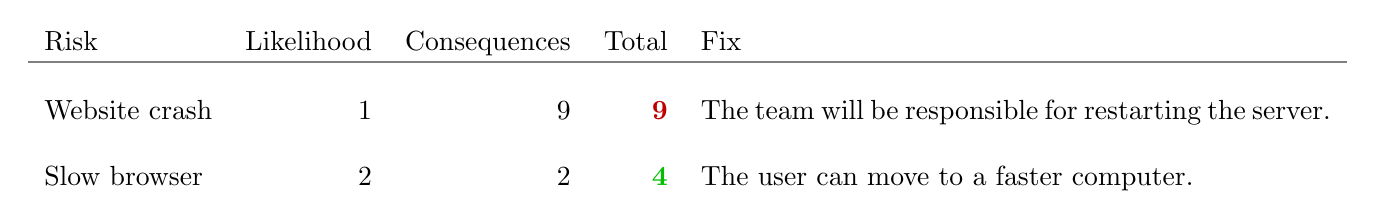
\begin{tikzpicture}
	\node[fill=white,inner sep=0pt] 
	{\rowcolors{1}{white}{white}
		\begin{tabular}{ l r r r p{8cm}  }
		Risk & Likelihood & Consequences & Total & Fix \\
		\arrayrulecolor{gray}\hline
		\arrayrulecolor{gray}\hline
		&\\
		Website crash & 1 & 9 & \textbf{\color{red!75!black!100}9} & The team will be responsible for restarting the server. \\
		&\\		
		Slow browser & 2 & 2 & \textbf{\color{green!75!black!100}4} & The user can move to a faster computer. \\
		
		\end{tabular}
	};
	
	
	\textbf{\color{green!75!black!100}3}
	\end{tikzpicture}
\end{table}

\newpage
\appendix
\section{Appendix}
\subsection{Design Concept}
A tentative conceptual design of the system is as followed:
\begin{center}
\tikzstyle{arrow}=[draw, -latex]
\begin{tikzpicture} [
	->,
	gray,
	>=stealth',
	task/.style={
		rectangle,
		draw,
		left color=white,
		right color=white,
        text=black,
        %font=\bfseries,
	}
	]
	\node [task, xshift=0ex, label={[align=center]SOCM}] (socm) {\SOCM}; 
	\node [task, xshift=5ex, label={[align=center]RoCM}, minimum width=2.5cm,right=of task2] (rocm) at (3,1) {\RoCM}; 
	\node [task, xshift=5ex, label={[align=center]RoCS}, minimum width=3cm,right=of task3] (rocs) at (3,-1) {\RoCS}; 
	
	\draw (socm) edge[out=0,in=180,->] (rocm);
	\draw (socm) edge[out=0,in=180,->] (rocs);
\end{tikzpicture}
\end{center}

\end{document}